% !TeX encoding = UTF-8
% !TeX program = xelatex
% !TeX spellcheck = <none>

\documentclass[degree=doctor,degree-type=academic,language=chinese]{thuthesis}
  % 学位 degree:
  %   doctor | master | bachelor | postdoc
  % 学位类型 degree-type:
  %   academic(默认)| professional
  % 语言 language
  %   chinese(默认)| english
  % 字体库 fontset
  %   windows | mac | fandol | ubuntu
  % 研究生院建议终版使用 Windows 平台的字体编译


% 论文基本配置,加载宏包等全局配置
% !TeX root = ./main.tex

% 论文基本信息配置

\thusetup{
  %******************************
  % 注意:
  %   1. 配置里面不要出现空行
  %   2. 不需要的配置信息可以删除
  %   3. 建议先阅读文档中所有关于选项的说明
  %******************************
  %
  % 输出格式
  %   选择打印版(print)或用于提交的电子版(electronic),前者会插入空白页以便直接双面打印
  %
  output = electronic,
  %
  % 标题
  %   可使用“\\”命令手动控制换行
  %
  title  = {低光照条件下的图像增强和识别\\关键技术研究},
  title* = {Research on Key Technologies of Image  Enhancement  and Recognition in Low-Light Conditions},
  % 
  institute = {华南理工大学},
  institute* = {South China University of Technology},
  %
  % 学位
  %   1. 学术型
  %      - 中文
  %        需注明所属的学科门类,例如:
  %        哲学、经济学、法学、教育学、文学、历史学、理学、工学、农学、医学、
  %        军事学、管理学、艺术学
  %      - 英文
  %        博士:Doctor of Philosophy
  %        硕士:
  %          哲学、文学、历史学、法学、教育学、艺术学门类,公共管理学科
  %          填写“Master of Arts“,其它填写“Master of Science”
  %   2. 专业型
  %      直接填写专业学位的名称,例如:
  %      教育博士、工程硕士等
  %      Doctor of Education, Master of Engineering
  %   3. 本科生不需要填写
  %
  degree-name  = {工学博士},
  degree-name* = {Doctor of Philosophy},
  %
  % 培养单位
  %   填写所属院系的全名
  %
  department = {计算机科学与工程学院},
  %
  % 学科
  %   1. 学术型学位
  %      获得一级学科授权的学科填写一级学科名称,其他填写二级学科名称
  %   2. 工程硕士
  %      工程领域名称
  %   3. 其他专业型学位
  %      不填写此项
  %   4. 本科生填写专业名称,第二学位论文需标注“(第二学位)”
  %
  discipline  = {计算机科学与技术},
  discipline* = {Computer Science and Technology},
  %
  % 姓名
  %
  author  = {梁锦秀},
  author* = {Liang Jinxiu},
  %
  % 指导教师
  %   中文姓名和职称之间以英文逗号“,”分开,下同
  %
  supervisor  = {许勇, 教授},
  supervisor* = {Professor Xu Yong},
  %
  % 副指导教师
  %
  %associate-supervisor  = {陈文光, 教授},
  %associate-supervisor* = {Professor Chen Wenguang},
  %
  % 联合指导教师
  %
  % co-supervisor  = {某某某, 教授},
  % co-supervisor* = {Professor Mou Moumou},
  %
  % 日期
  %   使用 ISO 格式;默认为当前时间
  %
   date = {2021-04-12},
  %
  % 是否在中文封面后的空白页生成书脊(默认 false)
  %
  include-spine = false,  
  %   
  % 是否使用pdf封面(默认 \@empty
  %
  include-cover = true,
  % cover-file = {figures/cover.pdf},
  %
  % 密级和年限
  %   秘密, 机密, 绝密
  %
  % secret-level = {秘密},
  % secret-year  = {10},
  %
  % 博士后专有部分
  %
  % clc                = {分类号},
  % udc                = {UDC},
  % id                 = {编号},
  % discipline-level-1 = {计算机科学与技术},  % 流动站(一级学科)名称
  % discipline-level-2 = {系统结构},          % 专业(二级学科)名称
  % start-date         = {2011-07-01},        % 研究工作起始时间
  toc-chapter-style = times,
  number-separator = {-},
  student-id = {xxxxxxx},
}

%---------------------------------------------------------------------------%
%->> Load packages 载入所需的宏包
%---------------------------------------------------------------------------%

% 定理类环境宏包
\usepackage{amsthm}
% 也可以使用 ntheorem
% \usepackage[amsmath,thmmarks,hyperref]{ntheorem}

\thusetup{
  %
  % 数学字体
  math-style = GB,  % GB | ISO | TeX
  math-font  = xits,  % sitx | xits | libertinus
}

% 可以使用 nomencl 生成符号和缩略语说明
% \usepackage{nomencl}
% \makenomenclature

% 表格加脚注
\usepackage{threeparttable}

% 表格中支持跨行
\usepackage{multirow}

% 固定宽度的表格。
% \usepackage{tabularx}

% 跨页表格
\usepackage{longtable}

% The package allows rows and columns to be coloured, and even individual cells.
\usepackage{colortbl}

% 量和单位
\usepackage{siunitx}

% 参考文献使用 BibTeX + natbib 宏包
% 顺序编码制
\usepackage[sort]{natbib}
\bibliographystyle{thuthesis-numeric}

% 参考文献中使用\citet{}时的引用方式
% \def\bibetal{等}
% \def\biband{和}

% Draw graphics directly with TeX commands
\usepackage{tikz}
\usepackage{pgfplots}% Create normal/logarithmic plots in two and three dimensions.
% \pgfplotsset{compat=1.17}
\usetikzlibrary{% load libraries
    positioning,
    arrows,
    calc,
    trees,
    spy
}%

% The package subfigure is now considered obsolete: it was superseded by subfig, but users may find the more recent subcaption package more satisfactory.
%\usepackage{subfigure}
%\usepackage{subfig}


% Draw dash-lines in array/tabular. 
\usepackage{arydshln}

% Marking things to do in a LaTeX document.
\usepackage[backgroundcolor=yellow]{todonotes}

% allow the placement of graphics relative to the “current position” using additional optional arguments of \includegraphics.
\usepackage{graphbox}
\usepackage{adjustbox}

%  provides an easy-to-use interface to the bbding symbol set
\usepackage{bbding}

% create algorithms
\usepackage{algorithm}
\usepackage[noend]{algpseudocode}

% hyperref 宏包在最后调用
\usepackage{hyperref}


%---------------------------------------------------------------------------%
%->> Configuration command
%---------------------------------------------------------------------------%

%-> Extensions and directories for graphics
% 定义所有的图片文件在 figures 子目录下
\graphicspath{{figures/}}

%- Declare graphic extensions for automatic selection when including graphics
%- via avoiding supplying graphic extensions in \includegraphics command,
%- the source file can be more general and adaptive
\DeclareGraphicsExtensions{.pdf,.png,.jpg,.eps,.tif,.bmp,.gif}%

% 数学命令
\makeatletter
\newcommand\dif{%  % 微分符号
  \mathop{}\!%
  \ifthu@math@style@TeX
    d%
  \else
    \mathrm{d}%
  \fi
}
\makeatother

% alignment in table
\renewcommand{\bfseries}{\fontseries{b}\selectfont}
\robustify\bfseries
\newrobustcmd{\BF}{\bfseries}

%-> Layout, space, and style
%\linespread{1.5}% 1.5 for "one and a half" line spacing, and 2.0 for "double" line spacing
%\setlength{\parskip}{0.5ex plus 0.25ex minus 0.25ex}% skip space a paragraph
% \setcounter{secnumdepth}{4}% depth for section numbering, default is 2(subsub)
% \setcounter{tocdepth}{2}% depth for the table of contents

\newcommand{\hiddensubsection}[1]{
	\stepcounter{subsection}
	\subsection*{{\rmfamily \arabic{chapter}.\arabic{section}.\arabic{subsection}}\hspace{1em}{#1}}
}

%---------------------------------------------------------------------------%
%->> User defined commands
%---------------------------------------------------------------------------%

%%Word abbreviations
% \newcommand{\st}{\text{s.t.}\ \ }
\newcommand\eg{\emph{e.g}~} 
\newcommand\Eg{\emph{E.g}~}
\newcommand\ie{\emph{i.e}~} 
\newcommand\Ie{\emph{I.e}~}
\newcommand\cf{\emph{c.f}~} 
\newcommand\Cf{\emph{C.f}~}
\newcommand\etc{\emph{etc}~} 
\newcommand\vsu{\emph{vs}~}
\newcommand\wrt{w.r.t~} 
\newcommand\dof{d.o.f~}
\newcommand\etal{\emph{et al}~}

%argmin and argmax
\DeclareMathOperator*{\argmin}{argmin}
\DeclareMathOperator*{\argmax}{argmax}


% Comments with highlights
\newcommand{\red}[1]{\textcolor[rgb]{1.00, 0.00, 0.00}{{#1}}} % comments in red
\newcommand{\green}[1]{\textcolor[rgb]{0.00, 1.00, 0.00}{{#1}}} % comments in green
\newcommand{\blue}[1]{\textcolor[rgb]{0.00, 0.00, 1.00}{{#1}}} % comments in blue
\newcommand{\black}[1]{\textcolor[rgb]{0.00, 0.00, 0.00}{{#1}}} % comments in black


%-> Math functions
%-
%- International standard layout rules (from isomath package)
%- The overall rule is that symbols representing math quantities or variables should
%- be italicised, symbols representing units or labels are unitalicised (roman).
%- Symbols for vectors and matrices are bold italic, symbols for tensors are 
%- sans-serif bold italic.
%- The above rules apply equally to letter symbols from the Greek and 
%- the Latin alphabet.
%- More information may be found in <<The LaTeX Mathematics Companion>>
%- However, math typefaces vary from field to field. To keep consistent typography
%- and easy adaption, it it always best to create a corresponding command for 
%- variables in each math category.  

%%Variable style
\newcommand{\vect}[1]{{\boldsymbol{#1}}} %%Vector in bold italic
\newcommand{\matx}[1]{{\boldsymbol{#1}}} %%Matrix in bold italic
\newcommand{\unitmt}[1]{\boldsymbol{\mathbf{#1}}} %%Identity matrix in bold roman
\newcommand{\tens}[1]{\boldsymbol{\mathsf{#1}}} %%Tensor in sans-serif bold italic
\newcommand{\unitts}[1]{\boldsymbol{\mathsf{#1}}}%%Identity tensor in sans-serif bold
\newcommand{\set}[1]{{\mathbb{#1}}}			%set notation
\newcommand{\opt}[1]{{\mathcal{#1}}}		%operator noation
\providecommand{\unit}[1]{\,\mathrm{#1}}% units in roman
\providecommand{\const}[1]{\mathrm{#1}}% math constants, functions
\providecommand{\desc}[1]{\mathrm{#1}}% descriptive superscripts and subscripts in roman type 
\providecommand{\div}{\operatorname{div}}% divergence operator
\providecommand{\order}{\operatorname{O}}% order operator
\providecommand{\trace}{\operatorname{tr}}% trace operator
\providecommand{\diag}{\operatorname{diag}}% diagonal
\providecommand{\def}{\operatorname{def}}% define

%%Variable abbreviations (vectors)
\newcommand{\va}{\vect{a}}
\newcommand{\vb}{\vect{b}}
\newcommand{\vc}{\vect{c}}
\newcommand{\vd}{\vect{d}}
\newcommand{\ve}{\vect{e}}
\newcommand{\vf}{\vect{f}}
\newcommand{\vg}{\vect{g}}
\newcommand{\vh}{\vect{h}}
\newcommand{\vi}{\vect{i}}
\newcommand{\vj}{\vect{j}}
\newcommand{\vk}{\vect{k}}
\newcommand{\vl}{\vect{l}}
\newcommand{\vell}{\vect{\ell}}
\newcommand{\vm}{\vect{m}}
\newcommand{\vn}{\vect{n}}
\newcommand{\vo}{\vect{o}}
\newcommand{\vp}{\vect{p}}
\newcommand{\vq}{\vect{q}}
\newcommand{\vr}{\vect{r}}
\newcommand{\vs}{\vect{s}}
\newcommand{\vt}{\vect{t}}
\newcommand{\vu}{\vect{u}}
\newcommand{\vv}{\vect{v}}
\newcommand{\vw}{\vect{w}}
\newcommand{\vx}{\vect{x}}
\newcommand{\vy}{\vect{y}}
\newcommand{\vz}{\vect{z}}
\newcommand{\valpha}{\vect{\alpha}}
\newcommand{\vbeta}{\vect{\beta}}
\newcommand{\vgamma}{\vect{\gamma}}
\newcommand{\vomega}{\vect{\omega}}
\newcommand{\vphi}{\vect{\phi}}
\newcommand{\vpsi}{\vect{\psi}}
\newcommand{\vtheta}{\vect{\theta}}
\newcommand{\vmu}{\vect{\mu}} 
\newcommand{\vepsilon}{\vect{\epsilon}}

%%Variable abbreviations (matrices)
\newcommand{\mA}{\matx{A}}
\newcommand{\mB}{\matx{B}}
\newcommand{\mC}{\matx{C}}
\newcommand{\mD}{\matx{D}}
\newcommand{\mE}{\matx{E}}
\newcommand{\mF}{\matx{F}}
\newcommand{\mG}{\matx{G}}
\newcommand{\mH}{\matx{H}}
\newcommand{\mI}{\matx{I}}
\newcommand{\mJ}{\matx{J}}
\newcommand{\mK}{\matx{K}}
\newcommand{\mL}{\matx{L}}
\newcommand{\mM}{\matx{M}}
\newcommand{\mN}{\matx{N}}
\newcommand{\mO}{\matx{O}}
\newcommand{\mP}{\matx{P}}
\newcommand{\mQ}{\matx{Q}}
\newcommand{\mR}{\matx{R}}
\newcommand{\mS}{\matx{S}}
\newcommand{\mT}{\matx{T}}
\newcommand{\mU}{\matx{U}}
\newcommand{\mV}{\matx{V}}
\newcommand{\mW}{\matx{W}}
\newcommand{\mX}{\matx{X}}
\newcommand{\mY}{\matx{Y}}
\newcommand{\mZ}{\matx{Z}}


\newcommand{\mGamma}{\matx{\Gamma}}
\newcommand{\mTheta}{\matx{\Theta}}
\newcommand{\mLambda}{\matx{\Lambda}}

%%Variable abbreviations (sets)
\newcommand{\sA}{\set{A}}
\newcommand{\sB}{\set{B}}
\newcommand{\sC}{\set{C}}
\newcommand{\sD}{\set{D}}
\newcommand{\sE}{\set{E}}
\newcommand{\sF}{\set{F}}
\newcommand{\sG}{\set{G}}
\newcommand{\sH}{\set{H}}
\newcommand{\sI}{\set{I}}
\newcommand{\sJ}{\set{J}}
\newcommand{\sK}{\set{K}}
\newcommand{\sL}{\set{L}}
\newcommand{\sM}{\set{M}}
\newcommand{\sN}{\set{N}}
\newcommand{\sO}{\set{O}}
\newcommand{\sP}{\set{P}}
\newcommand{\sQ}{\set{Q}}
\newcommand{\sR}{\set{R}}
\newcommand{\sS}{\set{S}}
\newcommand{\sT}{\set{T}}
\newcommand{\sU}{\set{U}}
\newcommand{\sV}{\set{V}}
\newcommand{\sW}{\set{W}}
\newcommand{\sX}{\set{X}}
\newcommand{\sY}{\set{Y}}
\newcommand{\sZ}{\set{Z}}

%%Variable abbreviations (operators)
\newcommand{\oA}{\opt{A}}
\newcommand{\oB}{\opt{B}}
\newcommand{\oC}{\opt{C}}
\newcommand{\oD}{\opt{D}}
\newcommand{\oE}{\opt{E}}
\newcommand{\oF}{\opt{F}}
\newcommand{\oG}{\opt{G}}
\newcommand{\oH}{\opt{H}}
\newcommand{\oI}{\opt{I}}
\newcommand{\oJ}{\opt{J}}
\newcommand{\oK}{\opt{K}}
\newcommand{\oL}{\opt{L}}
\newcommand{\oM}{\opt{M}}
\newcommand{\oN}{\opt{N}}
\newcommand{\oO}{\opt{O}}
\newcommand{\oP}{\opt{P}}
\newcommand{\oQ}{\opt{Q}}
\newcommand{\oR}{\opt{R}}
\newcommand{\oS}{\opt{S}}
\newcommand{\oT}{\opt{T}}
\newcommand{\oU}{\opt{U}}
\newcommand{\oV}{\opt{V}}
\newcommand{\oW}{\opt{W}}
\newcommand{\oX}{\opt{X}}
\newcommand{\oY}{\opt{Y}}
\newcommand{\oZ}{\opt{Z}}


\newif\ifblackandwhitecycle
\gdef\patternnumber{0}

\pgfkeys{/tikz/.cd,
	zoombox paths/.style={
		draw=orange,
		very thick
	},
	black and white/.is choice,
	black and white/.default=static,
	black and white/static/.style={
		draw=white,
		zoombox paths/.append style={
			draw=white,
			postaction={
				draw=black,
				loosely dashed
			}
		}
	},
	black and white/static/.code={
		\gdef\patternnumber{1}
	},
	black and white/cycle/.code={
		\blackandwhitecycletrue
		\gdef\patternnumber{1}
	},
	black and white pattern/.is choice,
	black and white pattern/0/.style={},
	black and white pattern/1/.style={
		draw=white,
		postaction={
			draw=black,
			dash pattern=on 1pt off 1pt
		}
	},
	black and white pattern/2/.style={
		draw=white,
		postaction={
			draw=black,
			dash pattern=on 2pt off 2pt
		}
	},
	black and white pattern/3/.style={
		draw=white,
		postaction={
			draw=black,
			dash pattern=on 2pt off 2pt on 1pt off 2pt
		}
	},
	black and white pattern/4/.style={
		draw=white,
		postaction={
			draw=black,
			dash pattern=on 2pt off 1pt on 1 pt off 1pt on 1 pt off 1pt
		}
	},
	zoomboxarray inner gap/.initial=2pt,
	zoomboxarray columns/.initial=2,
	zoomboxarray rows/.initial=2,
	subfigurename/.initial={},
	figurename/.initial={zoombox},
	zoomboxarray/.style={
		execute at begin picture={
			\begin{scope}[
				spy using outlines={%
					zoombox paths,
					width=\imagewidth / \pgfkeysvalueof{/tikz/zoomboxarray columns} - (\pgfkeysvalueof{/tikz/zoomboxarray columns} - 1) / \pgfkeysvalueof{/tikz/zoomboxarray columns} * \pgfkeysvalueof{/tikz/zoomboxarray inner gap} -\pgflinewidth,
					height=\imageheight/2 / \pgfkeysvalueof{/tikz/zoomboxarray rows} - (\pgfkeysvalueof{/tikz/zoomboxarray rows} - 1) / \pgfkeysvalueof{/tikz/zoomboxarray rows} * \pgfkeysvalueof{/tikz/zoomboxarray inner gap}-\pgflinewidth,
					magnification=3,
					every spy on node/.style={
						zoombox paths
					},
					every spy in node/.style={
						zoombox paths
					}
				}
				]
			},
		execute at end picture={
    		\end{scope}
    		% \node at (image.north) [anchor=north,inner sep=0pt] {\subcaptionbox{\label{\pgfkeysvalueof{/tikz/figurename}-image}}{\phantomimage}};
    		% \node at (zoomboxes container.north) [anchor=north,inner sep=0pt] {\subcaptionbox{\label{\pgfkeysvalueof{/tikz/figurename}-zoom}}{\phantomimage}};
    		\gdef\patternnumber{0}
		},
		spymargin/.initial=0.1em,
		zoomboxes xshift/.initial=1,
		zoomboxes right/.code=\pgfkeys{/tikz/zoomboxes xshift=1},
		zoomboxes left/.code=\pgfkeys{/tikz/zoomboxes xshift=-1},
		zoomboxes yshift/.initial=0,
		zoomboxes above/.code={
			\pgfkeys{/tikz/zoomboxes yshift=1},
			\pgfkeys{/tikz/zoomboxes xshift=0}
		},
		zoomboxes below/.code={
			\pgfkeys{/tikz/zoomboxes yshift=-1},
			\pgfkeys{/tikz/zoomboxes xshift=0}
		},
		% caption margin/.initial=4ex,
		caption margin/.initial=1pt,
	},
	adjust caption spacing/.code={},
	image container/.style={
		inner sep=0pt,
		at=(image.north),
		anchor=north,
		adjust caption spacing
	},
	zoomboxes container/.style={
		inner sep=0pt,
		at=(image.north),
		anchor=north,
		name=zoomboxes container,
		xshift=\pgfkeysvalueof{/tikz/zoomboxes xshift}*(\imagewidth+\pgfkeysvalueof{/tikz/spymargin}),
		yshift=\pgfkeysvalueof{/tikz/zoomboxes yshift}*(\imageheight+\pgfkeysvalueof{/tikz/spymargin}+\pgfkeysvalueof{/tikz/caption margin}),
		adjust caption spacing
	},
	calculate dimensions/.code={
		\pgfpointdiff{\pgfpointanchor{image}{south west} }{\pgfpointanchor{image}{north east} }
		\pgfgetlastxy{\imagewidth}{\imageheight}
		\global\let\imagewidth=\imagewidth
		\global\let\imageheight=\imageheight
		\gdef\columncount{1}
		\gdef\rowcount{1}
		\gdef\zoomboxcount{1}
	},
	image node/.style={
		inner sep=0pt,
		name=image,
		anchor=south west,
		append after command={
			[calculate dimensions]
			node [image container,subfigurename=\pgfkeysvalueof{/tikz/figurename}-image] {\phantomimage}
			node [zoomboxes container,subfigurename=\pgfkeysvalueof{/tikz/figurename}-zoom] {\phantomimage}
		}
	},
	color code/.style={
		zoombox paths/.append style={draw=#1}
	},
	connect zoomboxes/.style={
		spy connection path={\draw[draw=none,zoombox paths] (tikzspyonnode) -- (tikzspyinnode);}
	},
	help grid code/.code={
		\begin{scope}[
			x={(image.south east)},
			y={(image.north west)},
			font=\footnotesize,
			help lines,
			overlay
			]
			\foreach \x in {0,1,...,9} {
				\draw(\x/10,0) -- (\x/10,1);
				\node [anchor=north] at (\x/10,0) {0.\x};
			}
			\foreach \y in {0,1,...,9} {
				\draw(0,\y/10) -- (1,\y/10);                        \node [anchor=east] at (0,\y/10) {0.\y};
			}
		\end{scope}
	},
	help grid/.style={
		append after command={
			[help grid code]
		}
	},
}

\newcommand\phantomimage{%
	\phantom{%
		\rule{\imagewidth}{\imageheight/2}%
	}%
}
\newcommand\zoombox[2][]{
	\begin{scope}[zoombox paths]
		\pgfmathsetmacro\xpos{
			(\columncount-1)*(\imagewidth / \pgfkeysvalueof{/tikz/zoomboxarray columns} + \pgfkeysvalueof{/tikz/zoomboxarray inner gap} / \pgfkeysvalueof{/tikz/zoomboxarray columns} ) + \pgflinewidth
		}
		\pgfmathsetmacro\ypos{
			(\rowcount-1)*( \imageheight / \pgfkeysvalueof{/tikz/zoomboxarray rows} + \pgfkeysvalueof{/tikz/zoomboxarray inner gap} / \pgfkeysvalueof{/tikz/zoomboxarray rows} ) + 0.5*\pgflinewidth
		}
		\edef\dospy{\noexpand\spy [
			#1,
			zoombox paths/.append style={
				black and white pattern=\patternnumber
			},
			every spy on node/.append style={#1},
			x=\imagewidth,
			y=\imageheight
			] on (#2) in node [anchor=north west] at ($(zoomboxes container.north west)+(\xpos pt,-\ypos pt)$);}
		\dospy
		\pgfmathtruncatemacro\pgfmathresult{ifthenelse(\columncount==\pgfkeysvalueof{/tikz/zoomboxarray columns},\rowcount+1,\rowcount)}
		\global\let\rowcount=\pgfmathresult
		\pgfmathtruncatemacro\pgfmathresult{ifthenelse(\columncount==\pgfkeysvalueof{/tikz/zoomboxarray columns},1,\columncount+1)}
		\global\let\columncount=\pgfmathresult
		\ifblackandwhitecycle
		\pgfmathtruncatemacro{\newpatternnumber}{\patternnumber+1}
		\global\edef\patternnumber{\newpatternnumber}
		\fi
	\end{scope}
}



\begin{document}

% 封面
\maketitle                                                      % Uncomment!

% 学位论文指导小组、公开评阅人和答辩委员会名单
% % !TeX root = ../main.tex

\begin{committee}[name={学位论文指导小组、公开评阅人和答辩委员会名单}]

  \newcolumntype{C}[1]{@{}>{\centering\arraybackslash}p{#1}}

  \section*{指导小组名单}

  \begin{center}
    \begin{tabular}{C{3cm}C{3cm}C{9cm}@{}}
      李XX & 教授     & 清华大学 \\
      王XX & 副教授   & 清华大学 \\
      张XX & 助理教授 & 清华大学 \\
    \end{tabular}
  \end{center}


  \section*{公开评阅人名单}

  \begin{center}
    \begin{tabular}{C{3cm}C{3cm}C{9cm}@{}}
      刘XX & 教授   & 清华大学                    \\
      陈XX & 副教授 & XXXX大学                    \\
      杨XX & 研究员 & 中国XXXX科学院XXXXXXX研究所 \\
    \end{tabular}
  \end{center}


  \section*{答辩委员会名单}

  \begin{center}
    \begin{tabular}{C{2.75cm}C{2.98cm}C{4.63cm}C{4.63cm}@{}}
      主席 & 赵XX                  & 教授                    & 清华大学       \\
      委员 & 刘XX                  & 教授                    & 清华大学       \\
          & \multirow{2}{*}{杨XX} & \multirow{2}{*}{研究员} & 中国XXXX科学院 \\
          &                       &                         & XXXXXXX研究所  \\
          & 黄XX                  & 教授                    & XXXX大学       \\
          & 周XX                  & 副教授                  & XXXX大学       \\
      秘书 & 吴XX                  & 助理研究员              & 清华大学       \\
    \end{tabular}
  \end{center}

  
  % \clearpage
  % ~\\[1.5cm]
  % \begin{figure}\centering
  %   \includegraphics*[width=4.76in, height=1.08in, keepaspectratio=false]{scut_logo.png}
  % \end{figure}
  
  % \begin{center}\chuhao\bfseries\sffamily
  %     博士学位论文
  % \end{center}
  % ~\\[2.5cm]
  % \begin{longtable}{>{\centering}m{15.38cm}}\centering
  %   \erhao\sffamily 论文题目 \tabularnewline \hline
  %   \erhao\sffamily ~ \tabularnewline
  %   \erhao\sffamily ~ \tabularnewline \hline
  % \end{longtable}
  % ~\\[3cm]

  % \begin{longtable}{>{\centering}m{1.7in}>{\centering}m{1.8in}} \centering
  %   \makebox[6em][s]{作者姓名} &  \tabularnewline \cmidrule(lr){2-2} 
  %   \makebox[6em][s]{学科专业} &  \tabularnewline \cmidrule(lr){2-2} 
  %   \makebox[6em][s]{指导教师} &  \tabularnewline \cmidrule(lr){2-2}
  %   \makebox[6em][s]{所在学院} &  \tabularnewline \cmidrule(lr){2-2}
  %   \makebox[6em][s]{论文提交日期} &  \tabularnewline \cmidrule(lr){2-2} 
  % \end{longtable}
  
  
  % \clearpage
  
  % \noindent \textbf{Application of the Wavelet Analysis in}
  
  % \noindent \textbf{the Fault Diagnosis of Rotating Machines}
  % A Dissertation Submitted for the Degree of Doctor of Philosophy
  % \textbf{Candidate:Li Xiaoming}
  
  % \textbf{Supervisor:Prof. Chen Ping}
  
  
  % South China University of Technology 
  
  % Guangzhou, China
  
  % \clearpage
  
  % \noindent \textbf{分类号:                                        学校代号:10561}
  
  % \noindent \textbf{学 号:                                         秘密}$\mathrm{\bigstar}$\textbf{   5年}
  
  % \noindent 华南理工大学博士学位论文
  
  % \noindent \textbf{(论文题名和副题名)}
  
  % \noindent 作者姓名:                       指导教师姓名、职称: 
  
  % \noindent 申请学位级别:                   学科专业名称:
  
  % \noindent 研究方向:
  
  % \noindent 论文提交日期:     年   月   日      论文答辩日期:     年   月   日
  
  % \noindent 学位授予单位:华南理工大学           学位授予日期:     年   月   日
  
  % \noindent 答辩委员会成员:
  
  % \noindent 主席:\underbar{             } 
  
  % \noindent 委员:\underbar{                                                               }
  
  % \noindent 
  
  % \clearpage
  
  % \noindent \textbf{华南理工大学}
  
  % \noindent \textbf{学位论文原创性声明}
  
  % \noindent \textbf{}
  
  % 本人郑重声明:所呈交的论文是本人在导师的指导下独立进行研究所取得的研究成果。除了文中特别加以标注引用的内容外,本论文不包含任何其他个人或集体已经发表或撰写的成果作品。对本文的研究做出重要贡献的个人和集体,均已在文中以明确方式标明。本人完全意识到本声明的法律后果由本人承担。
  
  % 作者签名:                日期:    年   月   日
  
  % \noindent 
  
  % \noindent \textbf{学位论文版权使用授权书}
  
  % \noindent 
  
  % 本学位论文作者完全了解学校有关保留、使用学位论文的规定,即:研究生在校攻读学位期间论文工作的知识产权单位属华南理工大学。学校有权保存并向国家有关部门或机构送交论文的复印件和电子版,允许学位论文被查阅(除在保密期内的保密论文外);学校可以公布学位论文的全部或部分内容,可以允许采用影印、缩印或其它复制手段保存、汇编学位论文。本人电子文档的内容和纸质论文的内容相一致。
  
  % 本学位论文属于:
  
  % □保密(校保密委员会审定为涉密学位论文时间:\underbar{   }年\underbar{  }月\underbar{  }日),于\underbar{   }年\underbar{  }月\underbar{  }日解密后适用本授权书。
  
  % □不保密,同意在校园网上发布,供校内师生和与学校有共享协议的单位浏览;同意将本人学位论文编入有关数据库进行检索,传播学位论文的全部或部分内容。
  
  % (请在以上相应方框内打``$\mathrm{\sqrt{}}$'')
  
  
  
  % 作者签名:                        日期:
  
  % 指导教师签名:                    日期  
  
  % 作者联系电话:                    电子邮箱:
  
  % 联系地址(含邮编):
  
  

\end{committee}



% 也可以导入 Word 版转的 PDF 文件
% \begin{committee}[file=figures/committee.pdf]
% \end{committee}


% 使用授权的说明
% \copyrightpage
% 将签字扫描后授权文件 scan-copyright.pdf 替换原始页面
\copyrightpage[file=copyright.pdf]                              % Uncomment!

\frontmatter
% !TeX root = ../main.tex

% 中英文摘要和关键字

\begin{abstract}
  论文的摘要是对论文研究内容和成果的高度概括。
  摘要应对论文所研究的问题及其研究目的进行描述,对研究方法和过程进行简单介绍,对研究成果和所得结论进行概括。
  摘要应具有独立性和自明性,其内容应包含与论文全文同等量的主要信息。
  使读者即使不阅读全文,通过摘要就能了解论文的总体内容和主要成果。

  论文摘要的书写应力求精确、简明。
  切忌写成对论文书写内容进行提要的形式,尤其要避免“第 1 章……;第 2 章……;……”这种或类似的陈述方式。

  关键词是为了文献标引工作、用以表示全文主要内容信息的单词或术语。
  关键词不超过 5 个,每个关键词中间用分号分隔。

  % 关键词用“英文逗号”分隔,输出时会自动处理为正确的分隔符
  \thusetup{
    keywords = {关键词 1, 关键词 2, 关键词 3, 关键词 4, 关键词 5},
  }
\end{abstract}

\begin{abstract*}
  An abstract of a dissertation is a summary and extraction of research work and contributions.
  Included in an abstract should be description of research topic and research objective, brief introduction to methodology and research process, and summarization of conclusion and contributions of the research.
  An abstract should be characterized by independence and clarity and carry identical information with the dissertation.
  It should be such that the general idea and major contributions of the dissertation are conveyed without reading the dissertation.

  An abstract should be concise and to the point.
  It is a misunderstanding to make an abstract an outline of the dissertation and words “the first chapter”, “the second chapter” and the like should be avoided in the abstract.

  Keywords are terms used in a dissertation for indexing, reflecting core information of the dissertation.
  An abstract may contain a maximum of 5 keywords, with semi-colons used in between to separate one another.

  % Use comma as seperator when inputting
  \thusetup{
    keywords* = {keyword 1, keyword 2, keyword 3, keyword 4, keyword 5},
  }
\end{abstract*}

                                           % Uncomment!

% 目录
\tableofcontents                                                % Uncomment!

% 插图和附表清单
% \listoffiguresandtables  % 插图和附表清单
\listoffigures           % 插图清单                             % Uncomment!
\listoftables            % 附表清单                             % Uncomment!

% 符号对照表
% % !TeX root = ../main.tex

\begin{denotation}[3cm]
  \item[PI] 聚酰亚胺
  \item[MPI] 聚酰亚胺模型化合物,N-苯基邻苯酰亚胺
  \item[PBI] 聚苯并咪唑
  \item[MPBI] 聚苯并咪唑模型化合物,N-苯基苯并咪唑
  \item[PY] 聚吡咙
  \item[PMDA-BDA] 均苯四酸二酐与联苯四胺合成的聚吡咙薄膜
  \item[MPY] 聚吡咙模型化合物
  \item[As-PPT] 聚苯基不对称三嗪
  \item[MAsPPT] 聚苯基不对称三嗪单模型化合物,3,5,6-三苯基-1,2,4-三嗪
  \item[DMAsPPT] 聚苯基不对称三嗪双模型化合物(水解实验模型化合物)
  \item[S-PPT] 聚苯基对称三嗪
  \item[MSPPT] 聚苯基对称三嗪模型化合物,2,4,6-三苯基-1,3,5-三嗪
  \item[PPQ] 聚苯基喹噁啉
  \item[MPPQ] 聚苯基喹噁啉模型化合物,3,4-二苯基苯并二嗪
  \item[HMPI] 聚酰亚胺模型化合物的质子化产物
  \item[HMPY] 聚吡咙模型化合物的质子化产物
  \item[HMPBI] 聚苯并咪唑模型化合物的质子化产物
  \item[HMAsPPT] 聚苯基不对称三嗪模型化合物的质子化产物
  \item[HMSPPT] 聚苯基对称三嗪模型化合物的质子化产物
  \item[HMPPQ] 聚苯基喹噁啉模型化合物的质子化产物
  \item[PDT] 热分解温度
  \item[HPLC] 高效液相色谱(High Performance Liquid Chromatography)
  \item[HPCE] 高效毛细管电泳色谱(High Performance Capillary lectrophoresis)
  \item[LC-MS] 液相色谱-质谱联用(Liquid chromatography-Mass Spectrum)
  \item[TIC] 总离子浓度(Total Ion Content)
  \item[\textit{ab initio}] 基于第一原理的量子化学计算方法,常称从头算法
  \item[DFT] 密度泛函理论(Density Functional Theory)
  \item[$E_a$] 化学反应的活化能(Activation Energy)
  \item[ZPE] 零点振动能(Zero Vibration Energy)
  \item[PES] 势能面(Potential Energy Surface)
  \item[TS] 过渡态(Transition State)
  \item[TST] 过渡态理论(Transition State Theory)
  \item[$\increment G^\neq$] 活化自由能(Activation Free Energy)
  \item[$\kappa$] 传输系数(Transmission Coefficient)
  \item[IRC] 内禀反应坐标(Intrinsic Reaction Coordinates)
  \item[$\nu_i$] 虚频(Imaginary Frequency)
  \item[ONIOM] 分层算法(Our own N-layered Integrated molecular Orbital and molecular Mechanics)
  \item[SCF] 自洽场(Self-Consistent Field)
  \item[SCRF] 自洽反应场(Self-Consistent Reaction Field)
\end{denotation}



% 也可以使用 nomencl 宏包,需要在导言区
% \usepackage{nomencl}
% \makenomenclature

% 在这里输出符号说明
% \printnomenclature[3cm]

% 在正文中的任意为都可以标题
% \nomenclature{PI}{聚酰亚胺}
% \nomenclature{MPI}{聚酰亚胺模型化合物,N-苯基邻苯酰亚胺}
% \nomenclature{PBI}{聚苯并咪唑}
% \nomenclature{MPBI}{聚苯并咪唑模型化合物,N-苯基苯并咪唑}
% \nomenclature{PY}{聚吡咙}
% \nomenclature{PMDA-BDA}{均苯四酸二酐与联苯四胺合成的聚吡咙薄膜}
% \nomenclature{MPY}{聚吡咙模型化合物}
% \nomenclature{As-PPT}{聚苯基不对称三嗪}
% \nomenclature{MAsPPT}{聚苯基不对称三嗪单模型化合物,3,5,6-三苯基-1,2,4-三嗪}
% \nomenclature{DMAsPPT}{聚苯基不对称三嗪双模型化合物(水解实验模型化合物)}
% \nomenclature{S-PPT}{聚苯基对称三嗪}
% \nomenclature{MSPPT}{聚苯基对称三嗪模型化合物,2,4,6-三苯基-1,3,5-三嗪}
% \nomenclature{PPQ}{聚苯基喹噁啉}
% \nomenclature{MPPQ}{聚苯基喹噁啉模型化合物,3,4-二苯基苯并二嗪}
% \nomenclature{HMPI}{聚酰亚胺模型化合物的质子化产物}
% \nomenclature{HMPY}{聚吡咙模型化合物的质子化产物}
% \nomenclature{HMPBI}{聚苯并咪唑模型化合物的质子化产物}
% \nomenclature{HMAsPPT}{聚苯基不对称三嗪模型化合物的质子化产物}
% \nomenclature{HMSPPT}{聚苯基对称三嗪模型化合物的质子化产物}
% \nomenclature{HMPPQ}{聚苯基喹噁啉模型化合物的质子化产物}
% \nomenclature{PDT}{热分解温度}
% \nomenclature{HPLC}{高效液相色谱(High Performance Liquid Chromatography)}
% \nomenclature{HPCE}{高效毛细管电泳色谱(High Performance Capillary lectrophoresis)}
% \nomenclature{LC-MS}{液相色谱-质谱联用(Liquid chromatography-Mass Spectrum)}
% \nomenclature{TIC}{总离子浓度(Total Ion Content)}
% \nomenclature{\textit{ab initio}}{基于第一原理的量子化学计算方法,常称从头算法}
% \nomenclature{DFT}{密度泛函理论(Density Functional Theory)}
% \nomenclature{$E_a$}{化学反应的活化能(Activation Energy)}
% \nomenclature{ZPE}{零点振动能(Zero Vibration Energy)}
% \nomenclature{PES}{势能面(Potential Energy Surface)}
% \nomenclature{TS}{过渡态(Transition State)}
% \nomenclature{TST}{过渡态理论(Transition State Theory)}
% \nomenclature{$\increment G^\neq$}{活化自由能(Activation Free Energy)}
% \nomenclature{$\kappa$}{传输系数(Transmission Coefficient)}
% \nomenclature{IRC}{内禀反应坐标(Intrinsic Reaction Coordinates)}
% \nomenclature{$\nu_i$}{虚频(Imaginary Frequency)}
% \nomenclature{ONIOM}{分层算法(Our own N-layered Integrated molecular Orbital and molecular Mechanics)}
% \nomenclature{SCF}{自洽场(Self-Consistent Field)}
% \nomenclature{SCRF}{自洽反应场(Self-Consistent Reaction Field)}


% 待办事项表
% \listoftodos

% 正文部分
\mainmatter
% !TeX root = ../thuthesis-example.tex

\chapter{论文主要部分的写法}

研究生学位论文撰写,除表达形式上需要符合一定的格式要求外,内容方面上也要遵循一些共性原则。

通常研究生学位论文只能有一个主题(不能是几块工作拼凑在一起),该主题应针对某学科领域中的一个具体问题展开深入、系统的研究,并得出有价值的研究结论。
学位论文的研究主题切忌过大,例如,“中国国有企业改制问题研究”这样的研究主题过大,因为“国企改制”涉及的问题范围太广,很难在一本研究生学位论文中完全研究透彻。



\section{论文的语言及表述}

除国际研究生外,学位论文一律须用汉语书写。
学位论文应当用规范汉字进行撰写,除古汉语研究中涉及的古文字和参考文献中引用的外文文献之外,均采用简体汉字撰写。

国际研究生一般应以中文或英文书写学位论文,格式要求同上。
论文须用中文封面。

研究生学位论文是学术作品,因此其表述要严谨简明,重点突出,专业常识应简写或不写,做到立论正确、数据可靠、说明透彻、推理严谨、文字凝练、层次分明,避免使用文学性质的或带感情色彩的非学术性语言。

论文中如出现一个非通用性的新名词、新术语或新概念,需随即解释清楚。



\section{论文题目的写法}

论文题目应简明扼要地反映论文工作的主要内容,力求精炼、准确,切忌笼统。
论文题目是对研究对象的准确、具体描述,一般要在一定程度上体现研究结论,因此,论文题目不仅应告诉读者这本论文研究了什么问题,更要告诉读者这个研究得出的结论。
例如:“在事实与虚构之间:梅乐、卡彭特、沃尔夫的新闻观”就比“三个美国作家的新闻观研究”更专业、更准确。



\section{摘要的写法}

论文摘要是对论文研究内容的高度概括,应具有独立性和自含性,即应是 一篇简短但意义完整的文章。
通过阅读论文摘要,读者应该能够对论文的研究 方法及结论有一个整体性的了解,因此摘要的写法应力求精确简明。
论文摘要 应包括对问题及研究目的的描述、对使用的方法和研究过程进行的简要介绍、 对研究结论的高度凝练等,重点是结果和结论。

论文摘要切忌写成全文的提纲,尤其要避免“第 1 章……;第 2 章……;……”这样的陈述方式。



\section{引言的写法}

一篇学位论文的引言大致包含如下几个部分:
1、问题的提出;
2、选题背 景及意义;
3、文献综述;
4、研究方法;
5、论文结构安排。
\begin{itemize}
  \item 问题的提出:要清晰地阐述所要研究的问题“是什么”。
    \footnote{选题时切记要有“问题意识”,不要选不是问题的问题来研究。}
  \item 选题背景及意义:论述清楚为什么选择这个题目来研究,即阐述该研究对学科发展的贡献、对国计民生的理论与现实意义等。
  \item 文献综述:对本研究主题范围内的文献进行详尽的综合述评,“述”的同时一定要有“评”,指出现有研究状态,仍存在哪些尚待解决的问题,讲出自己的研究有哪些探索性内容。
  \item 研究方法:讲清论文所使用的学术研究方法。
  \item 论文结构安排:介绍本论文的写作结构安排。
\end{itemize}



\section{正文的写法}

本部分是论文作者的研究内容,不能将他人研究成果不加区分地掺和进来。
已经在引言的文献综述部分讲过的内容,这里不需要再重复。
各章之间要存在有机联系,符合逻辑顺序。



\section{结论的写法}

结论是对论文主要研究结果、论点的提炼与概括,应精炼、准确、完整,使读者看后能全面了解论文的意义、目的和工作内容。
结论是最终的、总体的结论,不是正文各章小结的简单重复。
结论应包括论文的核心观点,主要阐述作者的创造性工作及所取得的研究成果在本领域中的地位、作用和意义,交代研究工作的局限,提出未来工作的意见或建议。
同时,要严格区分自己取得的成果与指导教师及他人的学术成果。

在评价自己的研究工作成果时,要实事求是,除非有足够的证据表明自己的研究是“首次”、“领先”、“填补空白”的,否则应避免使用这些或类似词语。
                                           % Uncomment!
% !TeX root = ../thuthesis-example.tex

\chapter{图表示例}

\section{插图}

图片通常在 \env{figure} 环境中使用 \cs{includegraphics} 插入,如图~\ref{fig:example} 的源代码。
建议矢量图片使用 PDF 格式,比如数据可视化的绘图;
照片应使用 JPG 格式;
其他的栅格图应使用无损的 PNG 格式。
注意,LaTeX 不支持 TIFF 格式;EPS 格式已经过时。

\begin{figure}
  \centering
  
\includegraphics[width=0.6\linewidth]{example-image-a.pdf}
  \caption{示例图片}
  \label{fig:example}
\end{figure}

若图或表中有附注,采用英文小写字母顺序编号,附注写在图或表的下方。
% LaTeX 传统上一般将附注的内容同图表的标题写在一起,形成很长的一段文字。

如果一个图由两个或两个以上分图组成时,各分图分别以 (a)、(b)、(c)...... 作为图序,并须有分图题。
推荐使用 \pkg{subcaption} 宏包来处理, 比如图~\ref{fig:subfig-a} 和图~\ref{fig:subfig-b}。

\begin{figure}
  \centering
  \subcaptionbox{分图 A\label{fig:subfig-a}}
    {
\includegraphics[width=0.45\linewidth]{example-image-a.pdf}}
  \subcaptionbox{分图 B\label{fig:subfig-b}}
    {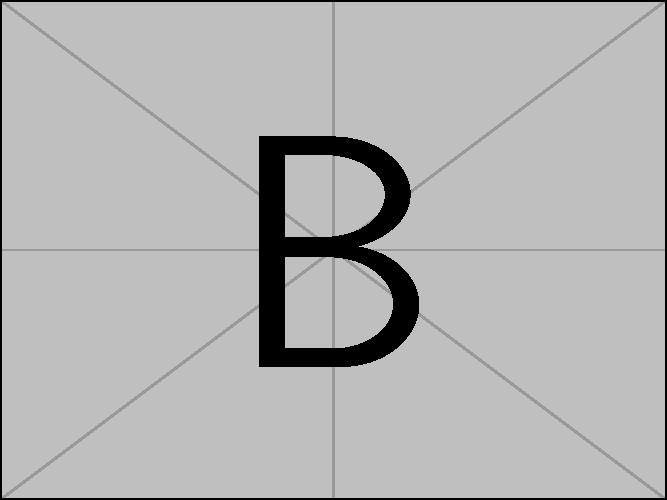
\includegraphics[width=0.45\linewidth]{example-image-b.pdf}}
  \caption{多个分图的示例}
  \label{fig:multi-image}
\end{figure}



\section{表格}

表应具有自明性。为使表格简洁易读,尽可能采用三线表,如表~\ref{tab:three-line}。
三条线可以使用 \pkg{booktabs} 宏包提供的命令生成。

\begin{table}
  \centering
  \caption{三线表示例}
  \begin{tabular}{ll}
    \toprule
    文件名          & 描述                         \\
    \midrule
    thuthesis.dtx   & 模板的源文件,包括文档和注释 \\
    thuthesis.cls   & 模板文件                     \\
    thuthesis-*.bst & BibTeX 参考文献表样式文件    \\
    thuthesis-*.bbx & BibLaTeX 参考文献表样式文件  \\
    thuthesis-*.cbx & BibLaTeX 引用样式文件        \\
    \bottomrule
  \end{tabular}
  \label{tab:three-line}
\end{table}

表格如果有附注,尤其是需要在表格中进行标注时,可以使用 \pkg{threeparttable} 宏包。
研究生要求使用英文小写字母 a、b、c……顺序编号,本科生使用圈码 ①、②、③……编号。

\begin{table}
  \centering
  \begin{threeparttable}[c]
    \caption{带附注的表格示例}
    \label{tab:three-part-table}
    \begin{tabular}{ll}
      \toprule
      文件名                 & 描述                         \\
      \midrule
      thuthesis.dtx\tnote{a} & 模板的源文件,包括文档和注释 \\
      thuthesis.cls\tnote{b} & 模板文件                     \\
      thuthesis-*.bst        & BibTeX 参考文献表样式文件    \\
      thuthesis-*.bbx        & BibLaTeX 参考文献表样式文件  \\
      thuthesis-*.cbx        & BibLaTeX 引用样式文件        \\
      \bottomrule
    \end{tabular}
    \begin{tablenotes}
      \item [a] 可以通过 xelatex 编译生成模板的使用说明文档;
        使用 xetex 编译 \file{thuthesis.ins} 时则会从 \file{.dtx} 中去除掉文档和注释,得到精简的 \file{.cls} 文件。
      \item [b] 更新模板时,一定要记得编译生成 \file{.cls} 文件,否则编译论文时载入的依然是旧版的模板。
    \end{tablenotes}
  \end{threeparttable}
\end{table}

如某个表需要转页接排,可以使用 \pkg{longtable} 宏包,需要在随后的各页上重复表的编号。
编号后跟表题(可省略)和“(续)”,置于表上方。续表均应重复表头。

\begin{longtable}{cccc}
    \caption{跨页长表格的表题} \\
    \toprule
    表头 1 & 表头 2 & 表头 3 & 表头 4 \\
    \midrule
  \endfirsthead
    \caption[]{跨页长表格的表题(续)} \\
    \toprule
    表头 1 & 表头 2 & 表头 3 & 表头 4 \\
    \midrule
  \endhead
    \bottomrule
  \endfoot
  Row 1  & & & \\
  Row 2  & & & \\
  Row 3  & & & \\
  Row 4  & & & \\
  Row 5  & & & \\
  Row 6  & & & \\
  Row 7  & & & \\
  Row 8  & & & \\
  Row 9  & & & \\
  Row 10 & & & \\
  Row 11 & & & \\
  Row 12 & & & \\
  Row 13 & & & \\
  Row 14 & & & \\
  Row 15 & & & \\
  Row 16 & & & \\
  Row 17 & & & \\
  Row 18 & & & \\
  Row 19 & & & \\
  Row 20 & & & \\
  Row 21 & & & \\
  Row 22 & & & \\
  Row 23 & & & \\
  Row 24 & & & \\
  Row 25 & & & \\
  Row 26 & & & \\
  Row 27 & & & \\
  Row 28 & & & \\
  Row 29 & & & \\
  Row 30 & & & \\
  Row 31 & & & \\
  Row 32 & & & \\
  Row 33 & & & \\
  Row 34 & & & \\
  Row 35 & & & \\
  Row 36 & & & \\
  Row 37 & & & \\
  Row 38 & & & \\
  Row 39 & & & \\
  Row 40 & & & \\
  Row 41 & & & \\
  Row 42 & & & \\
  Row 43 & & & \\
  Row 44 & & & \\
  Row 45 & & & \\
  Row 46 & & & \\
  Row 47 & & & \\
  Row 48 & & & \\
  Row 49 & & & \\
  Row 50 & & & \\
\end{longtable}
                                           % Uncomment!
% !TeX root = ../thuthesis-example.tex

\chapter{数学符号和公式}

\section{数学符号}

中文论文的数学符号默认遵循 GB/T 3102.11—1993《物理科学和技术中使用的数学符号》
\footnote{原 GB 3102.11—1993,自 2017 年 3 月 23 日起,该标准转为推荐性标准。}。
该标准参照采纳 ISO 31-11:1992 \footnote{目前已更新为 ISO 80000-2:2019。},
但是与 \TeX{} 默认的美国数学学会(AMS)的符号习惯有所区别。
具体地来说主要有以下差异:
\begin{enumerate}
  \item 大写希腊字母默认为斜体,如
    \begin{equation*}
      \Gamma \Delta \Theta \Lambda \Xi \Pi \Sigma \Upsilon \Phi \Psi \Omega.
    \end{equation*}
    注意有限增量符号 $\increment$ 固定使用正体,模板提供了 \cs{increment} 命令。
  \item 小于等于号和大于等于号使用倾斜的字形 $\le$、$\ge$。
  \item 积分号使用正体,比如 $\int$、$\oint$。
  \item 行间公式积分号的上下限位于积分号的上下两端,比如
    \begin{equation*}
      \int_a^b f(x) \dif x.
    \end{equation*}
    行内公式为了版面的美观,统一居右侧,如 $\int_a^b f(x) \dif x$ 。
  \item
    偏微分符号 $\partial$ 使用正体。
  \item
    省略号 \cs{dots} 按照中文的习惯固定居中,比如
    \begin{equation*}
      1, 2, \dots, n \quad 1 + 2 + \dots + n.
    \end{equation*}
  \item
    实部 $\Re$ 和虚部 $\Im$ 的字体使用罗马体。
\end{enumerate}

以上数学符号样式的差异可以在模板中统一设置。
另外国标还有一些与 AMS 不同的符号使用习惯,需要用户在写作时进行处理:
\begin{enumerate}
  \item 数学常数和特殊函数名用正体,如
    \begin{equation*}
      \uppi = 3.14\dots; \quad
      \symup{i}^2 = -1; \quad
      \symup{e} = \lim_{n \to \infty} \left( 1 + \frac{1}{n} \right)^n.
    \end{equation*}
  \item 微分号使用正体,比如 $\dif y / \dif x$。
  \item 向量、矩阵和张量用粗斜体(\cs{symbf}),如 $\symbf{x}$、$\symbf{\Sigma}$、$\symbfsf{T}$。
  \item 自然对数用 $\ln x$ 不用 $\log x$。
\end{enumerate}


英文论文的数学符号使用 \TeX{} 默认的样式。
如果有必要,也可以通过设置 \verb|math-style| 选择数学符号样式。

关于量和单位推荐使用
\href{http://mirrors.ctan.org/macros/latex/contrib/siunitx/siunitx.pdf}{\pkg{siunitx}}
宏包,
可以方便地处理希腊字母以及数字与单位之间的空白,
比如:
\SI{6.4e6}{m},
\SI{9}{\micro\meter},
\si{kg.m.s^{-1}},
\SIrange{10}{20}{\degreeCelsius}。



\section{数学公式}

数学公式可以使用 \env{equation} 和 \env{equation*} 环境。
注意数学公式的引用应前后带括号,建议使用 \cs{eqref} 命令,比如式 \eqref{eq:example}。
\begin{equation}
  \frac{1}{2 \uppi \symup{i}} \int_\gamma f = \sum_{k=1}^m n(\gamma; a_k) \mathscr{R}(f; a_k)
  \label{eq:example}
\end{equation}
注意公式编号的引用应含有圆括号,可以使用 \cs{eqref} 命令。

多行公式尽可能在“=”处对齐,推荐使用 \env{align} 环境。
\begin{align}
  a & = b + c + d + e \\
    & = f + g
\end{align}



\section{数学定理}

定理环境的格式可以使用 \pkg{amsthm} 或者 \pkg{ntheorem} 宏包配置。
用户在导言区载入这两者之一后,模板会自动配置 \env{thoerem}、\env{proof} 等环境。

\begin{theorem}[Lindeberg--Lévy 中心极限定理]
  设随机变量 $X_1, X_2, \dots, X_n$ 独立同分布, 且具有期望 $\mu$ 和有限的方差 $\sigma^2 \ne 0$,
  记 $\bar{X}_n = \frac{1}{n} \sum_{i+1}^n X_i$,则
  \begin{equation}
    \lim_{n \to \infty} P \left(\frac{\sqrt{n} \left( \bar{X}_n - \mu \right)}{\sigma} \le z \right) = \Phi(z),
  \end{equation}
  其中 $\Phi(z)$ 是标准正态分布的分布函数。
\end{theorem}
\begin{proof}
  Trivial.
\end{proof}

同时模板还提供了 \env{assumption}、\env{definition}、\env{proposition}、
\env{lemma}、\env{theorem}、\env{axiom}、\env{corollary}、\env{exercise}、
\env{example}、\env{remar}、\env{problem}、\env{conjecture} 这些相关的环境。
                                           % Uncomment!
% !TeX root = ../thuthesis-example.tex

\chapter{引用文献的标注}

模板支持 BibTeX 和 BibLaTeX 两种方式处理参考文献。
下文主要介绍 BibTeX 配合 \pkg{natbib} 宏包的主要使用方法。


\section{顺序编码制}

在顺序编码制下,默认的 \cs{cite} 命令同 \cs{citep} 一样,序号置于方括号中,
引文页码会放在括号外。
统一处引用的连续序号会自动用短横线连接。

\thusetup{
  cite-style = super,
}
\begin{tabular}{l@{\quad$\Rightarrow$\quad}l}
  \verb|\cite{zhangkun1994}|               & \cite{zhangkun1994}               \\
  \verb|\citet{zhangkun1994}|              & \citet{zhangkun1994}              \\
  \verb|\citep{zhangkun1994}|              & \citep{zhangkun1994}              \\
  \verb|\cite[42]{zhangkun1994}|           & \cite[42]{zhangkun1994}           \\
  \verb|\cite{zhangkun1994,zhukezhen1973}| & \cite{zhangkun1994,zhukezhen1973} \\
\end{tabular}


也可以取消上标格式,将数字序号作为文字的一部分。
建议全文统一使用相同的格式。

\thusetup{
  cite-style = inline,
}
\begin{tabular}{l@{\quad$\Rightarrow$\quad}l}
  \verb|\cite{zhangkun1994}|               & \cite{zhangkun1994}               \\
  \verb|\citet{zhangkun1994}|              & \citet{zhangkun1994}              \\
  \verb|\citep{zhangkun1994}|              & \citep{zhangkun1994}              \\
  \verb|\cite[42]{zhangkun1994}|           & \cite[42]{zhangkun1994}           \\
  \verb|\cite{zhangkun1994,zhukezhen1973}| & \cite{zhangkun1994,zhukezhen1973} \\
\end{tabular}



\section{著者-出版年制}

著者-出版年制下的 \cs{cite} 跟 \cs{citet} 一样。

\thusetup{
  cite-style = author-year,
}
\begin{tabular}{l@{\quad$\Rightarrow$\quad}l}
  \verb|\cite{zhangkun1994}|                & \cite{zhangkun1994}                \\
  \verb|\citet{zhangkun1994}|               & \citet{zhangkun1994}               \\
  \verb|\citep{zhangkun1994}|               & \citep{zhangkun1994}               \\
  \verb|\cite[42]{zhangkun1994}|            & \cite[42]{zhangkun1994}            \\
  \verb|\citep{zhangkun1994,zhukezhen1973}| & \citep{zhangkun1994,zhukezhen1973} \\
\end{tabular}

\vskip 2ex
\thusetup{
  cite-style = super,
}
注意,引文参考文献的每条都要在正文中标注
\cite{zhangkun1994,zhukezhen1973,dupont1974bone,zhengkaiqing1987,%
  jiangxizhou1980,jianduju1994,merkt1995rotational,mellinger1996laser,%
  bixon1996dynamics,mahui1995,carlson1981two,taylor1983scanning,%
  taylor1981study,shimizu1983laser,atkinson1982experimental,%
  kusch1975perturbations,guangxi1993,huosini1989guwu,wangfuzhi1865songlun,%
  zhaoyaodong1998xinshidai,biaozhunhua2002tushu,chubanzhuanye2004,%
  who1970factors,peebles2001probability,baishunong1998zhiwu,%
  weinstein1974pathogenic,hanjiren1985lun,dizhi1936dizhi,%
  tushuguan1957tushuguanxue,aaas1883science,fugang2000fengsha,%
  xiaoyu2001chubanye,oclc2000about,scitor2000project%
}。
                                           % Uncomment!

% 其他部分
\backmatter
% !TeX root = ../main.tex

\chapter{结{\quad}论}


\section*{研究工作总结}

结论是对论文主要研究结果、论点的提炼与概括,应精炼、准确、完整,使读者看后能全面了解论文的意义、目的和工作内容。
结论是最终的、总体的结论,不是正文各章小结的简单重复。
结论应包括论文的核心观点,主要阐述作者的创造性工作及所取得的研究成果在本领域中的地位、作用和意义,交代研究工作的局限,提出未来工作的意见或建议。
同时,要严格区分自己取得的成果与指导教师及他人的学术成果。
在评价自己的研究工作成果时,要实事求是,除非有足够的证据表明自己的研究是“首次”、“领先”、“填补空白”的,否则应避免使用这些或类似词语。

\section*{研究工作展望}

学位论文的结论单独作为一章排写,但不加章号。
结论是对整个论文主要成果的总结。在结论中应明确指出本研究内容的创造性成果或创新性理论(含新见解、新观点),对其应用前景和社会、经济价值等加以预测和评价,并指出今后进一步在本研究方向进行研究工作的展望与设想。
如果不能导出应有的结论,也可以没有结论而进行必要的讨论。
                                         % Uncomment!

% 参考文献
\bibliography{ref/refs}  % 参考文献使用 BibTeX 编译             % Uncomment!
% \printbibliography       % 参考文献使用 BibLaTeX 编译

% 附录
% \appendix
% % !TeX root = ../main.tex

\chapter{补充内容}

附录是与论文内容密切相关、但编入正文又影响整篇论文编排的条理和逻辑性的资料,例如某些重要的数据表格、计算程序、统计表等,是论文主体的补充内容,可根据需要设置。


\section{图表示例}

\subsection{图}

附录中的图片示例(图~\ref{fig:appendix-figure})。

\begin{figure}
  \centering
  
\includegraphics[width=0.6\linewidth]{example-image-a.pdf}
  \caption{附录中的图片示例}
  \label{fig:appendix-figure}
\end{figure}


\subsection{表格}

附录中的表格示例(表~\ref{tab:appendix-table})。

\begin{table}
  \centering
  \caption{附录中的表格示例}
  \begin{tabular}{ll}
    \toprule
    文件名          & 描述                         \\
    \midrule
    thuthesis.dtx   & 模板的源文件,包括文档和注释 \\
    thuthesis.cls   & 模板文件                     \\
    thuthesis-*.bst & BibTeX 参考文献表样式文件    \\
    thuthesis-*.bbx & BibLaTeX 参考文献表样式文件  \\
    thuthesis-*.cbx & BibLaTeX 引用样式文件        \\
    \bottomrule
  \end{tabular}
  \label{tab:appendix-table}
\end{table}


\section{数学公式}

附录中的数学公式示例(公式~\eqref{eq:appendix-equation})。
\begin{equation}
  \frac{1}{2 \uppi \symup{i}} \int_\gamma f = \sum_{k=1}^m n(\gamma; a_k) \mathscr{R}(f; a_k)
  \label{eq:appendix-equation}
\end{equation}


% 个人简历、在学期间完成的相关学术成果
% !TeX root = ../main.tex

\begin{resume}[name={攻读博士学位期间取得的研究成果}]

  已发表(包括已接受待发表)的论文,以及已投稿、或已成文打算投稿、或拟成文投稿的论文情况\textbf{\underbar{(只填写与学位论文内容相关的部分):}}
  \begin{table}
    \centering{}%
    \small 
    \begin{tabular}{|>{\centering}m{0.5cm}|>{\centering}m{2.3cm}|>{\centering}m{3.2cm}|>{\centering}m{2.8cm}|>{\centering}m{1.5cm}|>{\centering}m{1.5cm}|>{\centering}m{1cm}|}
      \hline 
      序号 & 作者(全体作者,按顺序排列) & 题 \quad 目 						   & 发表或投稿刊物名称、级别 & 发表的卷期、年月、页码 & 相当于学位论文的哪一部分(章、节) & 被索引收录情况\tabularnewline
      \hline 
      1    & Author A, Author B 	  & Title & IEEE Transactions on XXX, JCR-1区期刊  & 已投稿 & 第X章& 无    \tabularnewline
      \hline 
      2    & Author A, Author B 	  & Title & IEEE Transactions on XXX, JCR-1区期刊  & 已投稿 & 第X章& 无    \tabularnewline
      \hline 
      3    & Author A, Author B 	  & Title & IEEE Transactions on XXX, JCR-1区期刊  & 已投稿 & 第X章& 无    \tabularnewline
      \hline 
      4    & Author A, Author B 	  & Title & IEEE Transactions on XXX, JCR-1区期刊  & 已投稿 & 第X章& 无    \tabularnewline
      \hline 

    \end{tabular}
  \end{table}
  
  注:在“发表的卷期、年月、页码”栏:
  
  1.如果论文已发表,请填写发表的卷期、年月、页码;
  
  2.如果论文已被接受,填写将要发表的卷期、年月;
  
  3.以上都不是,请据实填写“已投稿”,“拟投稿”。
  
  不够请另加页。
  
%   二、与学位内容相关的其它成果(包括专利、著作、获奖项目等)

\end{resume}


% % 也可以导入 Word 版转的 PDF 文件
% \begin{resume}[file=figures/achievements.pdf]
% \end{resume}
                                             % Uncomment!

% 致谢
% !TeX root = ../main.tex

\begin{acknowledgements}
    衷心感谢导师×××教授和物理系××副教授对本人的精心指导。他们的言传身教将使我终生受益。

    在美国麻省理工学院化学系进行九个月的合作研究期间,承蒙 Robert Field 教授热心指导与帮助,不胜感激。
  
    感谢×××××实验室主任×××教授,以及实验室全体老师和同窗们学的热情帮助和支持!
  
    本课题承蒙国家自然科学基金资助,特此致谢。
\end{acknowledgements}
                                   % Uncomment!

% % 答辩委员会决议书  
% !TeX root = ../main.tex

% \begin{resolution}[name={答辩委员签名的答辩决议书}]
%     \noindent \textbf{Ⅳ - 2答辩委员会对论文的评定意见}


%     \begin{table}
%         \begin{longtable}{|m{1.20cm}|m{13.80cm}|}
%             \hline
%             \multicolumn{2}{|m{15.00cm}|}{
%                 论文提出了……

%                 论文取得的主要创新性成果包括:

%                 1. ……

%                 2. ……

%                 3. ……

%                 论文工作表明作者在×××××具有×××××知识,具有××××能力,论文××××,答辩××××。

%                 答辩委员会表决,(×票/一致)同意通过论文答辩,并建议授予×××(姓名)×××(门类)学博士学位。
%             } \tabularnewline[10.00cm] \hline 
%             \multicolumn{2}{|m{15.00cm}|}{\begin{tabular}{l}
%                 论文答辩日期:\underbar{\ \ \ \ \ \ \ \ \ \ \ \ \ \ \ \ }年\underbar{\ \ \ \ \ \ \ \ }月\underbar{\ \ \ \ \ \ \ \ }日 \\
%                 答辩委员会委员共\_\_\_\_\_\_\_人,到会委员\_\_\_\_\_\_\_人 \\
%                  表决票数:优秀(  )票;良好(  )票;及格(  )票;不及格(  )票 \\
%                   表决结果(打``$\mathrm{\sqrt{}}$''):优秀(  );良好(  );及格(  );不及格(  )   \\ 
%                决议:同意授予博士学位(  )   不同意授予博士学位(  )
%             \end{tabular}} \tabularnewline[2.00cm] \hline 
%             答辩委员会成员签名 & 
%             \begin{tabular}{b{4.60cm}b{4.60cm}b{4.60cm}}
%                 & & \\
%                 \underbar{\ \ \ \ \ \ \ \ \ \ \ \ \ \ \ \ \ \ \ \ (主席)}  &
%                 \underbar{\ \ \ \ \ \ \ \ \ \ \ \ \ \ \ \ \ \ \ \ \ \ \ \ \ \ \ \ \ \ \ \ \ \ \ \ }   &
%                 \underbar{\ \ \ \ \ \ \ \ \ \ \ \ \ \ \ \ \ \ \ \ \ \ \ \ \ \ \ \ \ \ \ \ \ \ \ \ }  \\
%                 & & \\
%                 \underbar{\ \ \ \ \ \ \ \ \ \ \ \ \ \ \ \ \ \ \ \ \ \ \ \ \ \ \ \ \ \ \ \ \ \ \ \ }   & 
%                 \underbar{\ \ \ \ \ \ \ \ \ \ \ \ \ \ \ \ \ \ \ \ \ \ \ \ \ \ \ \ \ \ \ \ \ \ \ \ }  &
%                 \underbar{\ \ \ \ \ \ \ \ \ \ \ \ \ \ \ \ \ \ \ \ \ \ \ \ \ \ \ \ \ \ \ \ \ \ \ \ }  \\
%             \end{tabular} \tabularnewline \hline
%         \end{longtable}
%     \end{table}

% \end{resolution}





% 也可以导入 Word 版转的 PDF 文件
\begin{committee}[file=figures/resolution.pdf]
\end{committee}
                                         % Uncomment!

\end{document}
